\documentclass[10pt,letterpaper]{article}
\usepackage[T1]{fontenc}
\usepackage[utf8]{inputenc}
\usepackage[margin=0.9in]{geometry}
\usepackage{mathptmx,courier,amsmath,amssymb,amsthm,booktabs,longtable,array,graphicx}
\usepackage[hidelinks]{hyperref}
\usepackage{microtype}
\graphicspath{{../figures_next/}{../figures/}}
\newtheorem{theorem}{Theorem}
\newtheorem{corollary}{Corollary}
\newcommand{\CLARA}{\textsc{Clara}}
\newcommand{\SampleCount}{6,210}
\newcommand{\PatientCount}{6,204}
\newcommand{\ProfiledSampleCount}{5,924}
\newcommand{\PrimarySampleCount}{5,841}
\newcommand{\InterpretationCount}{5,760}
\newcommand{\ContrastCount}{1,440}
\newcommand{\SensitiveContrastCount}{428}
\newcommand{\SensitiveFamilyCount}{323}
\newcommand{\OptimalQuestions}{1.149}
\newcommand{\FixedQuestions}{1.238}
\newcommand{\FixedSaving}{7.2}

\title{\CLARA{}: Technical Supplement\\Shared Completions, Full Proofs, and Complete Evidence}
\author{Pratyush Kumar Shukla, Manveer Singh Tib, and Siddhant Garg}
\date{7 October 2026}
\begin{document}
\maketitle
\noindent This supplement provides full proofs and execution details for the IEEE-format paper. TCGA computations, a separately frozen MSK-IMPACT stress test, mathematical/software checks, and stipulated policy scenarios are distinct evidence classes. The complete source package retains all registry rows and raw public inputs.

\section{Model and executable semantics}
For one cohort--gene family, let $S_r$ denote patient $r$'s specimens and $E$ its gene-appropriate profiled membership set. Specification $i$ chooses counting unit, assay denominator, specimen context, and consequence set. Set $A_i$ to its context specimens and $H_i=A_i\cap E$ in profiled mode, otherwise $H_i=A_i$. Let $B_s$ and $T_s$ be the recorded broad/restricted class-set indicators of profiled specimen $s$, with $T_s\leq B_s$. An unprofiled specimen's indicators come from $z_s\in\{0,1,2\}$: $B_s=\mathbf1[z_s\geq1]$, $T_s=\mathbf1[z_s=2]$.

The denominator and completed positive numerator are
\begin{align}
 n_i&=\begin{cases}|H_i|,&\text{specimen mode},\\|\{r:S_r\cap H_i\ne\varnothing\}|,&\text{patient mode},\end{cases}\\
 k_i(z)&=\begin{cases}\sum_{s\in H_i} e_{is}(z_s),&\text{specimen mode},\\
 \sum_r\mathbf1[\exists s\in S_r\cap H_i:e_{is}(z_s)=1],&\text{patient mode},\end{cases}
\end{align}
where $e_{is}$ selects $B_s$ or $T_s$ according to $i$. Profiled mode never includes an unprofiled specimen's latent indicator. The observed execution is the all-zero missing completion. Projection to patient identifiers follows context and profile filtering; deduplication is by the scientific counting unit, not mutation-record rows.

\subsection{Partially observed patients}
A patient can have both profiled and unprofiled specimens. Suppose a profiled primary specimen is recorded negative and an unprofiled metastatic specimen becomes positive. In patient/cohort/all mode this patient contributes one; in patient/profiled/all or patient/cohort/primary mode it remains negative. If instead the profiled specimen is already positive, the missing specimen cannot add another patient positive but can add a specimen positive. Patient-block enumeration preserves all of these distinctions, including partial observation within a patient.

The universe of missing specimen states is fixed for the family and shared across all alternatives. Clarifying a field changes the surviving specifications, not the unknown specimen statuses. Analysis is per gene: this model does not impose cross-gene co-occurrence constraints or statistical exchangeability of event statuses.

\subsection{Consequence sets and assumptions}
{\raggedright The broad set is \texttt{Missense\_Mutation}, \texttt{Nonsense\_Mutation}, \texttt{Frame\_Shift\_Del}, \texttt{Frame\_Shift\_Ins}, \texttt{In\_Frame\_Del}, \texttt{In\_Frame\_Ins}, \texttt{Splice\_Site}, \texttt{Translation\_Start\_Site}, and \texttt{Nonstop\_Mutation}. The restricted set removes missense and the two in-frame labels. It includes start-loss and stop-loss labels, so we report it as restricted rather than a literal protein-truncating-variant set. The protocol and software use the internal token \texttt{truncating} for this exact class set. Unlisted labels are excluded, including 111 TCGA \texttt{Splice\_Region} records in the frozen panel data. These are source-record classes, not verified pathogenic or loss-of-function labels.\par}

Profile membership supplies an assay-record eligibility contract. We hold recorded profiled event labels fixed and allow only unprofiled statuses to vary. No technical false-negative model, per-base sensitivity model, or biological prevalence prior is asserted. Data outside the panel, unavailable specimens, and errors in specimen or patient identifiers are outside the certificate. The Cartesian completion space permits any combination of local states; valid external constraints would require a new support computation or restricted block sets.

\section{Sharp support and identification proofs}
Partition unknown statuses by patient. Let $\mathcal Z_r=\{0,1,2\}^{m_r}$ and let $k_{ir}(z_r)$ be the patient block's contribution. Fixed known contributions form $k_i^0$. Then $f_i(z)=c_i+\sum_r v_{ir}(z_r)$, with $c_i=k_i^0/n_i$ and $v_{ir}=k_{ir}/n_i$.

\begin{theorem}[Separable shared support]
For any real $a,b$ and a finite Cartesian completion space,
\[
 H_{ij}(a,b)=\max_{z\in\prod_r\mathcal Z_r}(af_i(z)+bf_j(z))
 =ac_i+bc_j+\sum_r\max_{u\in\mathcal Z_r}(av_{ir}(u)+bv_{jr}(u)).
\]
Every support value is attained by a feasible shared completion.
\end{theorem}
\begin{proof}
For any $z$, each block term is at most its own maximum, giving the right side as an upper bound. Because each block is finite, choose an argmax $u_r^*$ in every block. Their product $z^*=(u_r^*)_r$ belongs to the Cartesian space and attains every local maximum simultaneously. This proves equality and supplies a witness. Empty collections of unknown blocks reduce to the fixed contribution; the argument still holds.
\end{proof}

\begin{corollary}[Absolute discrepancy and marginal endpoints]
$A_{ij}=100\max\{H_{ij}(1,-1),H_{ji}(1,-1)\}$ is sharp. Likewise $L_i=c_i+\sum_r\min v_{ir}$ and $U_i=c_i+\sum_r\max v_{ir}$ are sharp endpoints.
\end{corollary}
The corollary follows by taking the two possible directions of an absolute value and applying the theorem. A pair's maximum discrepancy may use a different completion from another pair's maximum; certifying \emph{all} pairs bounds each pair in \emph{every} world and does not require one world to realize all maxima together.

The outer-box bound is $A^{\rm box}_{ij}=100\max\{U_i-L_j,U_j-L_i\}$. It is an upper bound since the actual pair is always inside its marginal box. It need not be attainable. If $f_i(z)=f_j(z)$ for every $z$ but $L_i<U_i$, sharp discrepancy is zero while the box permits $100(U_i-L_i)$. Completion equivalence is exactly $A_{ij}=0$. The favorable equivalence-merged box comparator removes all such paired alarms before planning.

\subsection{Partial observation can make the box loose beyond equivalence}
In OV--BRCA1, patient/cohort/all/broad (index 4) and patient/cohort/primary/broad (index 6) have different denominators but share their 62 missing specimens. The sharp absolute discrepancy is 0.046913 pp, while the box permits 10.645204 pp. Their largest relative discrepancy is 0.00342466, below the primary 0.10 threshold. They are not equivalent functions, so the equivalence-merged baseline still retains its infeasible alarm. This illustrative case is not a separately sampled validation item; it comes from the fully retained registry.

\section{Fractional optimization and strict threshold labels}
Let $p(z)=f_i(z)$, $q(z)=f_j(z)$, and $s(z)=(p(z)+q(z))/2+\epsilon>0$. Consider the positive directed ratio maximum $r^+=\max\{0,\max_z(p-q)/s\}$. Define $\Phi(\rho)=\max_z[(p-q)-\rho s]$. The support theorem computes this function through coefficients $(1-\rho/2,-1-\rho/2)$ and the constant $-\rho\epsilon$.

\begin{theorem}[Parametric characterization]
If $\max_z(p-q)>0$, $\Phi$ has one zero $r^+\in(0,2)$, equal to the largest directed ratio. If $\max_z(p-q)\leq0$, the positive directed maximum is zero. The sharp absolute relative discrepancy is the larger positive directional maximum.
\end{theorem}
\begin{proof}
For any $\rho$, $\Phi(\rho)>0$ iff some $z$ satisfies $(p-q)/s>\rho$; similarly $\Phi(\rho)\leq0$ iff every ratio is at most $\rho$. The finite maximum of affine functions is continuous. For $\rho_2>\rho_1$, $s(z)\geq\epsilon$ implies
\[
 \Phi(\rho_2)\leq\Phi(\rho_1)-(\rho_2-\rho_1)\epsilon,
\]
so it is strictly decreasing. In the positive case, $\Phi(0)>0$; at $\rho=2$, $(p-q)-2s=-2q-2\epsilon<0$. Thus a unique zero exists in $(0,2)$ and equals the largest feasible ratio. If the directed numerator is never positive, its positive part is zero. Any nonzero absolute difference is positive in one direction; maximizing both directions proves the final statement. This is an application of the classical fractional-programming relation \cite{dinkelbach}, not a claim of a new general optimization principle.
\end{proof}

Forty bisection iterations have nominal interval width $2/2^{40}$. Floating-point brackets are checked against directly enumerated small-world ratios within $3\times10^{-12}$; they are numerical reporting intervals, not statistical confidence intervals or interval-arithmetic proofs. Primary and tolerance-grid classification instead use exact rational decisions.

For $\tau=a/b$ and integer positive-unit counts $k_i,k_j$, a directed ratio exceeds $\tau$ iff
\begin{align}
 \frac{k_i/n_i-k_j/n_j}{(k_i/n_i+k_j/n_j)/2+\epsilon}&>a/b\\
 \iff (2b-a)k_i n_j-(2b+a)k_j n_i&>2a\epsilon n_i n_j.
\end{align}
Maximize the integer left side by patient block and compare it using \texttt{Fraction} for the recorded decimal $\epsilon$. Reverse the direction and take the maximum. For an absolute threshold $\beta$ pp, the corresponding support $M^{\rm abs}$ violates iff $100M^{\rm abs}>\beta n_i n_j$. At $\beta=5$, this is $20M^{\rm abs}>n_i n_j$. Scientific counts in these snapshots fit signed 64-bit integer arithmetic; the implementation is not a promise for arbitrary count magnitudes.

An adversarial cutoff fixture uses $p=21/40$, $q=19/40$. Their absolute difference is exactly 5 pp; their relative discrepancy is strictly less than 0.1 because of $\epsilon$. Neither strict primary cutoff is exceeded. Naive binary floating subtraction can represent their difference above 0.05 and incorrectly flag the absolute branch. The count-support test preserves the declared rule. A separate fixture violates only the absolute criterion, verifying the OR combination rather than assuming relative and absolute branches are interchangeable.

\section{Semantic graph, policy optimality, and point guard}
Define the undirected graph $G$ with an edge iff a paired absolute or relative maximum exceeds its threshold. For any surviving $C$, stability is equivalent to $G[C]$ having no edge. Every subset of a stable $C$ is stable. A truthful field reply retains the intended candidate and deletes incompatible vertices; it cannot create a new edge. This monotonicity certifies stopping inside the declared candidate and completion spaces, not correctness of an unseen natural-language interpretation.

\subsection{Expected and minimax policies}
Let $w(C)=\sum_{i\in C}w_i>0$ and $p_{qv}=w(C_{qv})/w(C)$. For a stable state, $V(C)=W(C)=0$. Otherwise
\[
 V(C)=\min_q\{c_q+\sum_vp_{qv}V(C_{qv})\},\qquad
 W(C)=\min_q\{c_q+\max_vW(C_{qv})\}.
\]
\begin{theorem}[Conditional decision-tree optimum]
These recurrences attain the minimum expected and maximum-path costs, respectively, among truthful field-question trees with the graph stopping rule and positive field costs.
\end{theorem}
\begin{proof}
Induct on the number of unresolved fields. A stable state can stop with zero cost; positive costs rule out an improvement by asking another question. A nonstable state with all fields resolved is impossible because a singleton has no graph edge. Every nonterminal tree therefore has an admissible first field. Its conditional children have fewer unresolved fields, and replacing either child with an optimal subtree cannot increase the corresponding expected or worst-case objective. Optimizing the first field gives the recurrence. Conversely each recurrence choice followed by its optimal child policies is a realizable tree attaining that value. This is a specialization of classical optimal identification planning \cite{garey}.
\end{proof}

For four binary fields, each partial assignment has values unresolved/zero/one, so there are at most $3^4=81$ states, including singleton leaves. Policies ask at most four questions. Equal-cost uniform planning has dyadic branch probabilities; the sensitivity grid is evaluated numerically with positive product priors. Path costs agree with Bellman values, and every terminal subset is checked independently against its graph.

The one-step edge heuristic uses conditional pair mass
\[
 e(C)=\sum_{i<j\in C}\frac{w_iw_j}{w(C)^2}\mathbf1[(i,j)\in E_G]
\]
and maximizes $(e(C)-\sum_vp_{qv}e(C_{qv}))/c_q$. Entropy-only splitting maximizes $-\sum_vp_{qv}\log_2p_{qv}/c_q$. Their tie-breaking order is unit, assay, context, class. All 24 fixed field permutations skip nonvarying fields and stop using the same chosen graph. Hindsight best global and per-family orders are both reported; no oracle order is represented as a deployed learned policy.

\subsection{Point-answer impossibility for a fixed missing target}
Let $L(C)=\min_iL_i$, $U(C)=\max_iU_i$. The endpoint values are feasible for some candidate--world pairs. For any proposed $x$, at least one endpoint error is at least $(U(C)-L(C))/2$ by the triangle inequality. The midpoint achieves that radius for every feasible value, proving the minimax formula. A point answer within $\eta$ is possible iff $U(C)-L(C)\leq2\eta$. Even the most refined intent set, a singleton, can fail this condition. Clarification that preserves the fixed selected estimand cannot reduce its missing-status interval; additional measurements or valid constraints are required. The published question-count analyses optimize semantic stopping only, while point availability is reported separately.

\section{Primary TCGA registry and verification}
The fixed 30-gene panel is TP53, KRAS, PIK3CA, PTEN, APC, BRAF, NRAS, NF1, EGFR, ARID1A, KDM6A, NOTCH1, RB1, CDKN2A, FBXW7, CTNNB1, ATM, BRCA1, BRCA2, SMAD4, STK11, KEAP1, ERBB2, FGFR3, GATA3, SPOP, FOXA1, IDH1, VHL, and SETD2. Every cohort--gene family, including zero-event families, is retained.

TCGA PanCancer Atlas sources \cite{cerami,gao,hoadley} were retrieved through the public cBioPortal API between 06:34:24 and 06:35:40 UTC on 6 October 2026. The 38 raw JSON files total 14,079,113 bytes. The portal reported software v7.1.2 and database software 3.0.0; these are not immutable data-revision identifiers. Raw hashes, request parameters, retrieval times, normalization, and a local protocol lock preserve the exact used inputs. Retrieval was sequential, not atomic. The original pre-download protocol and later completion-extension protocol are separate, locally timestamped records rather than public preregistrations.

\begin{center}\small\begin{tabular}{lrrrrrr}
\toprule
Cohort & Specimens & Patients & Unprofiled & Sensitive & Box-only & Beyond equiv.\\
\midrule
BLCA & 411 & 411 & 1 & 30/30 & 180 & 0\\
BRCA & 1,084 & 1,084 & 18 & 30/30 & 348 & 0\\
COADREAD & 594 & 594 & 60 & 30/30 & 360 & 0\\
HNSC & 523 & 523 & 8 & 30/30 & 324 & 0\\
LUAD & 566 & 566 & 0 & 30/30 & 0 & 0\\
PRAD & 494 & 494 & 0 & 26/30 & 0 & 0\\
SKCM & 448 & 442 & 8 & 30/30 & 116 & 57\\
UCEC & 529 & 529 & 12 & 30/30 & 318 & 0\\
ACC & 92 & 92 & 1 & 30/30 & 342 & 0\\
KIRC & 512 & 512 & 110 & 30/30 & 360 & 0\\
LIHC & 372 & 372 & 6 & 30/30 & 348 & 0\\
OV & 585 & 585 & 62 & 30/30 & 352 & 232\\
\bottomrule
\end{tabular}
\end{center}

The primary TCGA results are 323 observed-sensitive families and 356 completion-sensitive families. Pair counts are 23,370 observed, 31,337 sharp coupled, 34,385 raw box, and 31,626 equivalence-merged box. Among 3,048 raw-box-only alarms, 2,759 are removed by exact function equivalence and 289 reflect dependence beyond equivalence. The latter comprise 232 OV pairs and 57 SKCM pairs. This denominator should accompany any percentage reduction, since equivalence explains most raw-box improvement.

\subsection{Independent global support verification}
TCGA has at most one unprofiled specimen per patient. Write that specimen's broad/restricted indicators as $0\leq t_s\leq b_s\leq1$. A patient OR is either already positive (constant), unaffected by this specimen (constant), or equal to the corresponding indicator. Thus every selected fraction is affine in these indicators. The feasible product of triangular polytopes has only $(0,0),(1,0),(1,1)$ vertices per specimen, making every linear support optimum realizable by discrete event states.

\texttt{verify\_completion\_lp.py} independently constructs these global affine expressions directly from specimen metadata and recorded mutations, without using the local contribution tables. Global SciPy/HiGHS linear programs compare directed absolute supports and the relative threshold supports to exact local integer values for all 43,200 paired cases. Zero terms and identical objective structures are cached: 363 distinct objectives, 172,437 repeated requests. This checks support decisions, not independent biological truth. It is specific to the affine TCGA case; the general repeated-unprofiled OR case is checked by exhaustive small-world fixtures.

The 18 completion/planning contracts include partially profiled patients, context intersections, unprofiled source positives, nested classes, repeated unprofiled specimens, full-world absolute and relative oracles, exact cutoff equality, an absolute-only violation, undefined denominators, singleton point nonidentification, irrelevant entropy splits, nonuniform weights, unequal costs, batch/scalar Bellman agreement, worst-case minimax paths, and domination of all fixed orders. The 16 counting contracts also pass. Sixty-four seeded fixtures (seed 20261006) contain at most three unknown specimens and enumerate 1,314 global completions. They provide mathematical/software coverage, not an additional empirical sample size.

\section{Complete policy and tolerance results}
Uniform priors weight the 16 field assignments, not distinct numerical values. Equal costs measure abstract field questions, not time, usability, or willingness to answer. The sharp coupled expected optimum is 1.773263889; the per-family fixed optimum and edge-greedy mean match it. The best global order averages 1.830208333. Minimax mean is 1.818055556 with worst path four questions. Entropy-only mean is 3.845833333. The raw box optimum is 2.496875000 and merged-box optimum is 1.833333333. Coupling saves 28.981\% versus raw-box planning and 3.277\% versus equivalence-merged-box planning.

\begin{figure}[ht]
\centering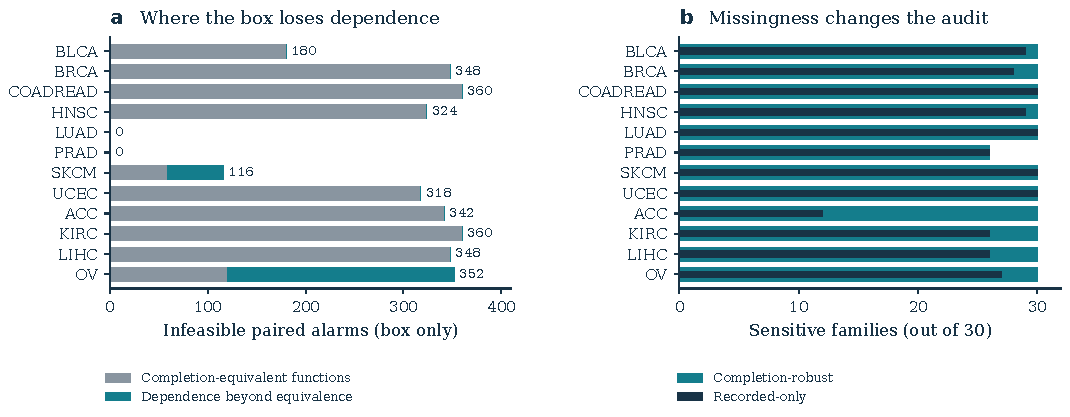
\includegraphics[width=\textwidth]{05_coupling_audit.pdf}
\caption{Additional dependency and missingness audits. The left panel partitions all box-only pair alarms into completion-equivalent functions and dependence beyond equivalence; both are infeasible under the shared model. The right panel reports sensitive family counts by cohort. These are fully retained, clustered deterministic summaries, not independent pairwise observations.}
\end{figure}

The intent-prior grid assigns each field-zero probability independently from $\{0.2,0.5,0.8\}$, giving 81 priors. Costs are $(1,1,1,1)$, $(1,1,1,3)$, or $(1,3,3,1)$. The archive includes 87,480 family--prior--cost records and 243 aggregate scenario records. Savings versus the best global fixed order span 0.6947--7.2873\%; savings versus per-family fixed orders span numerical zero--0.0964\%. Small negative floating residuals of magnitude $2.2\times10^{-16}$ are zero to numerical precision. No human behavior distribution is inferred from this grid.

\begin{figure}[ht]
\centering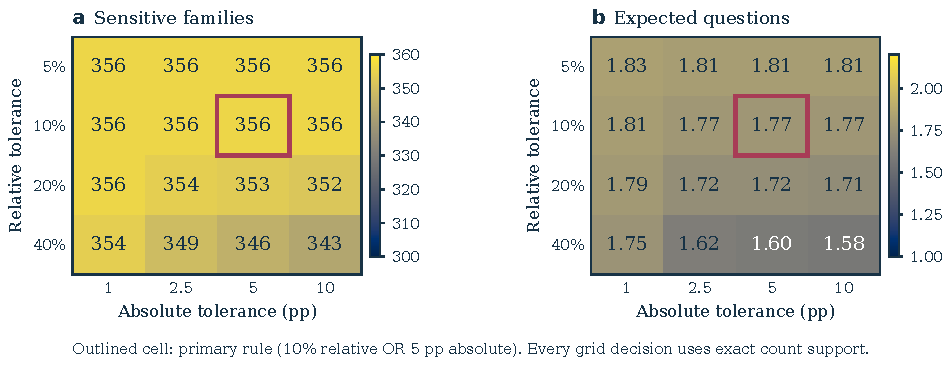
\includegraphics[width=\textwidth]{07_tolerances.pdf}
\caption{The full prespecified tolerance grid. Primary thresholds are outlined. All 5,760 family--threshold scenarios use exact count-support labels. At these thresholds the robust sensitive-family count ranges from 343 to 356; mean optimal questions range from 1.577 to 1.828. Low-frequency genes can violate the relative criterion at small absolute changes; tolerances express engineering choices rather than biological significance.}
\end{figure}

\section{Separate targeted-assay stress test}
The unchanged gene list is applied to MSK-IMPACT 2017 \cite{zehir}. Clinical specimen metadata, mutations, panel matrix, and authoritative IMPACT341/410 gene sets are pinned to DataHub commit \texttt{dca75cb3f32b82d54a6f78bf0a6323e5b}\allowbreak\texttt{975aca1}. Each large-file download matches the commit's Git LFS content SHA-256 and byte count. The public LFS service advertised by the repository configuration supplies content unavailable through a media mirror. Transient signed download URLs are not retained. Source/adapted MSK data retain their source ODbL license and attribution.

The source has 10,945 specimens, 10,336 patients, 6,213 primary specimens, 4,731 metastasis specimens, and one unspecified specimen type. There are 562 repeated-specimen patients: 519 with two, 40 with three, two with four, and one with five specimens. The mutation file has 78,220 records over all source genes and 21,807 records in the fixed panel. IMPACT410 covers 8,136 specimens and IMPACT341 covers 2,809. Every selected gene is in both panels, so all 328,350 specimen--gene eligibility cells are profiled. The adapter nonetheless explicitly checks gene-panel membership instead of assuming that a mutation absence means assay eligibility.

The primary context is exactly \texttt{SAMPLE\_TYPE=Primary}. The unspecified type is retained in all-specimen analyses and excluded from the primary restriction without imputation. Both engines match all 480 specifications. Observed, coupled, box, and merged-box graphs coincide because no selected gene has an unprofiled specimen. All 30 families are sensitive; reference class/context/unit/assay sensitive counts are 30/8/0/0. The largest reference unit difference is 0.551761 pp and 4.923979\% relative. All fixed selected intervals are singletons, so no 2.5 pp point guard fails. The exact, greedy, best global fixed, and best per-family fixed means are all 1.500; entropy-only uses four questions. These negative efficiency and missing-eligibility findings limit the extension's claims.

\begin{center}\small\begin{longtable}{lrrrr}
\toprule
Gene & Unit flip (pp) & Unit flip (relative) & Semantic diameter (pp) & Mean questions\\
\midrule
\endhead
TP53 & 0.488 & 0.0117 & 28.20 & 1.500\\
KRAS & 0.552 & 0.0362 & 15.47 & 1.500\\
PIK3CA & 0.159 & 0.0127 & 12.39 & 1.500\\
PTEN & 0.039 & 0.0064 & 2.67 & 1.500\\
APC & 0.352 & 0.0338 & 3.30 & 2.000\\
BRAF & 0.004 & 0.0007 & 4.95 & 1.500\\
NRAS & 0.116 & 0.0492 & 2.33 & 2.000\\
NF1 & 0.172 & 0.0315 & 2.38 & 1.000\\
EGFR & 0.103 & 0.0178 & 6.07 & 1.500\\
ARID1A & 0.268 & 0.0330 & 2.31 & 1.000\\
KDM6A & 0.099 & 0.0308 & 1.55 & 2.000\\
NOTCH1 & 0.106 & 0.0256 & 3.02 & 1.000\\
RB1 & 0.121 & 0.0255 & 1.15 & 1.000\\
CDKN2A & 0.157 & 0.0358 & 2.18 & 1.000\\
FBXW7 & 0.059 & 0.0187 & 2.69 & 2.000\\
CTNNB1 & 0.051 & 0.0161 & 3.05 & 1.000\\
ATM & 0.151 & 0.0306 & 3.31 & 1.500\\
BRCA1 & 0.087 & 0.0433 & 1.61 & 1.000\\
BRCA2 & 0.079 & 0.0215 & 2.41 & 1.500\\
SMAD4 & 0.125 & 0.0290 & 2.95 & 2.000\\
STK11 & 0.055 & 0.0161 & 1.47 & 1.000\\
KEAP1 & 0.101 & 0.0311 & 2.60 & 2.000\\
ERBB2 & 0.009 & 0.0032 & 2.88 & 1.500\\
FGFR3 & 0.011 & 0.0053 & 2.43 & 2.000\\
GATA3 & 0.021 & 0.0079 & 1.38 & 2.000\\
SPOP & 0.056 & 0.0429 & 1.32 & 1.500\\
FOXA1 & 0.068 & 0.0339 & 1.70 & 2.000\\
IDH1 & 0.028 & 0.0095 & 4.12 & 2.000\\
VHL & 0.002 & 0.0013 & 0.93 & 1.000\\
SETD2 & 0.062 & 0.0147 & 2.18 & 1.000\\
\bottomrule
\end{longtable}
\end{center}

This clinical study is evaluated separately from TCGA, with no pooled cancer-frequency estimate or claim of known disjoint individual patients across resources. It challenges specimen aggregation and a targeted-assay adapter within the same curation ecosystem; it does not empirically validate repeated \emph{unprofiled} blocks, a language interface, or a clinical recommendation.

\section{Serial scalability protocol and complete configurations}
The extension protocol \texttt{scale\_protocol.json} was hashed and locally recorded before measurements. It adds engineering evaluation after the primary registry results; it is not public preregistration. The host exposes an AMD EPYC 9V74 80-Core Processor. One serial Python 3.12.14 process uses NumPy 2.3.5; no worker pool or accelerator is used. The container shares a host, so timings are descriptive engineering measurements rather than statistically independent performance samples.

The cohort list uses its unchanged protocol order; the gene list uses the fixed order printed above. Cohort scaling retains the first 1/3/6/12 cohorts and all 30 genes. Gene scaling retains all 12 cohorts and the first 1/5/10/20/30 genes. Each configuration has one untimed warmup followed by five measurements, with configuration order randomized using seed 20261007. The two full-registry endpoints occur separately in that randomized schedule; their differing medians reflect ordinary run variation, not different scientific inputs. Each job recomputes the strict-threshold graph, all-pairs absolute support, 40-step relative bounds, and the uniform expected-cost planner from prepared tables. It excludes network access, parsing, baseline query execution, model preparation, independent LP checks, and file/figure writing. All retained models contain 25,740 ungrouped local states and 338 distinct contribution tables summed across families. Preparation of the 360 models takes 20.561 s separately; full per-cohort preparation rows are retained.

\begin{center}\small\begin{tabular}{llrrr}
\toprule
Axis & Cohorts $\times$ genes & Families & Median (s) & Min--max (s)\\
\midrule
Cohorts & 1$\times$30 & 30 & 0.089 & 0.086--0.097\\
Cohorts & 3$\times$30 & 90 & 0.326 & 0.302--0.370\\
Cohorts & 6$\times$30 & 180 & 0.556 & 0.498--0.591\\
Cohorts & 12$\times$30 & 360 & 1.040 & 1.009--1.175\\
Genes & 12$\times$1 & 12 & 0.036 & 0.034--0.037\\
Genes & 12$\times$5 & 60 & 0.185 & 0.182--0.189\\
Genes & 12$\times$10 & 120 & 0.372 & 0.348--0.444\\
Genes & 12$\times$20 & 240 & 0.712 & 0.669--0.715\\
Genes & 12$\times$30 & 360 & 1.099 & 1.005--1.246\\
\bottomrule
\end{tabular}
\end{center}

\subsection{Synthetic block-count and local-block workloads}
Identical-table scaling uses 10/100/1,000/10,000/100,000 independent one-unknown patient blocks, with all specimens primary and a recorded-negative profiled specimen per patient. The same $3\times16$ table is either repeated in a loop or stored once with exact integer multiplicity. Denominators scale with patient count. The timed operation is one all-pairs integer support with coefficients 19 and $-21$. Grouped/ungrouped supports agree exactly at every count. Ungrouped medians are 0.091/0.956/10.093/97.225/897.703 ms; grouped medians remain 0.014--0.015 ms. These timings exclude grouping construction and storage of the original patient records. Constant grouped \emph{kernel} time in this favorable workload does not imply constant end-to-end time or space as records grow.

The local-block workload instead places 1--10 unprofiled primary specimens in one patient with one recorded-negative profiled specimen. Each of its $3^m$ nested states is explicitly enumerated. Local sample contributions count positives; patient contributions take an OR. Table construction and the same support call are measured separately. This demonstrates the retained local exponential limit. At 10 unknown specimens the table uses 7.21 MiB, while support temporaries require additional memory; the implementation's 100,000-state enumeration budget refuses 11 unknown specimens. No scalability row is a new biological cohort or portal-wide result.

\begin{center}\small\begin{tabular}{rrrrr}
\toprule
Unknowns & Local states & Table (MiB) & Build (ms) & Support (ms)\\
\midrule
1 & 3 & 0.0004 & 0.056 & 0.015\\
2 & 9 & 0.0011 & 0.026 & 0.020\\
3 & 27 & 0.0033 & 0.030 & 0.028\\
4 & 81 & 0.0099 & 0.043 & 0.057\\
5 & 243 & 0.0297 & 0.098 & 0.159\\
6 & 729 & 0.0890 & 0.298 & 0.435\\
7 & 2,187 & 0.2670 & 0.941 & 1.922\\
8 & 6,561 & 0.8009 & 3.995 & 6.920\\
9 & 19,683 & 2.4027 & 10.654 & 21.957\\
10 & 59,049 & 7.2081 & 30.851 & 64.814\\
\bottomrule
\end{tabular}
\end{center}

\begin{figure}[ht]
\centering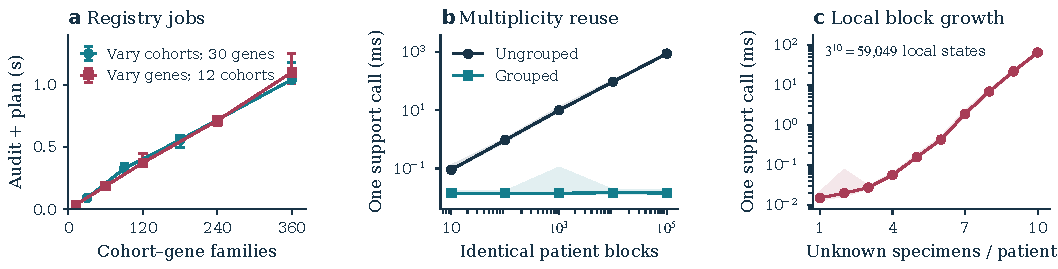
\includegraphics[width=\textwidth]{09_scaling.pdf}
\caption{Complete serial scaling evaluation. Medians and observed min--max ranges are descriptive measurements over five repetitions. The prepared-table registry job and synthetic single-support kernels time different operations. Grouping exploits identical contribution tables; local unknown multiplicity still incurs exponential enumeration.}
\end{figure}

Independent cohort--gene jobs suggest a distributed map stage, followed by aggregation of family receipts. Each worker would require the same hashed snapshot, class-set/schema contract, model, and tolerance definitions; failures or stale inputs must invalidate a certificate. Data retrieval, panel harmonization, patient-identifier collisions, load skew, and large local blocks would remain separate bottlenecks. This is an execution design sketch, not a measured HPC deployment or a claim about all cBioPortal studies.

\section{Typed guard, provenance receipts, and evidence acquisition}
\texttt{guard\_demo.py --demo} executes three supplied typed KIRC--VHL requests. An unconstrained request has status \texttt{clarification\_\allowbreak required}. Fixing cohort denominator, all specimens, and broad class, with unit unresolved, yields \texttt{interval\_answer}: $[166,276]/512$ with no point value. Fixing patient/profiled/all/broad yields \texttt{point\_answer\_\allowbreak with\_\allowbreak certificate}: $166/402$. This demonstrates downstream-agent decision branches; no LLM or natural-language candidate generator is invoked.

Each JSON receipt binds the request, frozen snapshot contents, scientific protocols, implementation, exact tolerances, candidate set, sharp discrepancies, graph stopping decision, and point guard. Canonical SHA-256 values detect changed content and support exact replay. A basic JSON-LD PROV-O graph \cite{prov} connects input snapshot entities, the audit activity, and its result. This is query-level lineage metadata, not tuple-level why/where or semiring provenance \cite{buneman,green}, a digital signature, or evidence that the original data are accurate. All three demonstrations pass full reconstruction and replay. Nine interface contracts test statuses, point suppression, replay, modified answers/bindings, unsupported fields/values, and nonfinite budgets, in addition to the existing 34 contracts.

For the fixed KIRC--VHL broad cohort target, measuring $t$ of the 110 unknown patients leaves a worst-case radius $(110-t)/(2\cdot512)$ regardless of measured outcomes. At least 85 additional measurements are sufficient and necessary for a \emph{guaranteed} radius at most 2.5 pp under this unrestricted assay-record model. A global cap $c$ on unknown broad positives instead gives the conditional interval $[166,166+c]/512$; the executed cap sensitivity uses $c=0,10,25,26,50,110$. The cap 25 meets the point budget; 26 does not. These assumptions are hypothetical, not frequency estimates from matched cohorts. External evidence would need an explicit applicability and assay-error model. Global constraints couple patients and therefore require a constrained support optimizer instead of unrestricted separable local maxima.

\section{Reproduction and evidence boundaries}
\texttt{python reproducibility/run\_all.py} performs offline verification, rebuilds the observed-only comparison registry, recomputes shared completions and independent support checks, executes the tolerance grid and MSK adapter, and regenerates vector figures and data tables. LaTeX documents and poster/guide/atlas have separate build commands documented in the README. The executed notebook supplies a short inspection path for tests, paired certificates, policy scenarios, and the central matrix. Raw inputs, protocol records, full result registries, figure code, and editable manuscript sources are included; no public repository URL is invented.

A mathematical certificate is conditional on the declared supported functions and feasible worlds. Neither counting-engine agreement, support-optimum agreement, synthetic fixtures, nor exhaustive hypothetical intent paths validates clinical biology, a language generator, complete interpretation coverage, or actual researcher burden. No statistical significance tests are attached to correlated family--pair counts. Main-text operational tolerances and stipulated costs are unchanged from their recorded analysis specifications.

\section*{AI disclosure}
OpenAI ChatGPT (Codex) assisted in drafting, restructuring, proofs, software, data analysis, and figure design throughout this supplement and the associated package. Numerical findings were computed from preserved public data or explicitly labeled mathematical/software fixtures. The authors remain responsible for validation and the final submission.
\begin{thebibliography}{99}
\bibitem{nalir} F. Li and H. V. Jagadish, ``Constructing an interactive natural language interface for relational databases,'' \emph{Proc. VLDB Endow.}, vol. 8, no. 1, pp. 73--84, 2014, doi: 10.14778/2735461.2735468.
\bibitem{ambiqt} A. Bhaskar, T. Tomar, A. Sathe, and S. Sarawagi, ``Benchmarking and improving text-to-SQL generation under ambiguity,'' in \emph{Proc. EMNLP}, 2023, pp. 7053--7074, doi: 10.18653/v1/2023.emnlp-main.436.
\bibitem{saparina} I. Saparina and M. Lapata, ``Disambiguate first, parse later: Generating interpretations for ambiguity resolution in semantic parsing,'' in \emph{Findings of ACL}, 2025, pp. 16825--16839, doi: 10.18653/v1/2025.findings-acl.863.
\bibitem{intentsim} M. J. Q. Zhang and E. Choi, ``Clarify when necessary: Resolving ambiguity through interaction with LMs,'' in \emph{Findings of NAACL}, 2025, pp. 5541--5558, doi: 10.18653/v1/2025.findings-naacl.306.
\bibitem{sage} M. Suri, P. Mathur, N. Lipka, F. Dernoncourt, R. A. Rossi, and D. Manocha, ``Structured uncertainty guided clarification for LLM agents,'' in \emph{Findings of ACL}, 2026, pp. 40811--40838, doi: 10.18653/v1/2026.findings-acl.2028.
\bibitem{incomplete} T. Imieli\'nski and W. Lipski, Jr., ``Incomplete information in relational databases,'' \emph{J. ACM}, vol. 31, no. 4, pp. 761--791, 1984, doi: 10.1145/1634.1886.
\bibitem{dinkelbach} W. Dinkelbach, ``On nonlinear fractional programming,'' \emph{Management Science}, vol. 13, no. 7, pp. 492--498, 1967, doi: 10.1287/mnsc.13.7.492.
\bibitem{garey} M. R. Garey, ``Optimal binary identification procedures,'' \emph{SIAM J. Appl. Math.}, vol. 23, no. 2, pp. 173--186, 1972, doi: 10.1137/0123019.
\bibitem{manski} C. F. Manski, \emph{Partial Identification of Probability Distributions}. New York, NY, USA: Springer, 2003, doi: 10.1007/b97478.
\bibitem{console} M. Console, L. Libkin, and L. Peterfreund, ``Querying incomplete numerical data: Between certain and possible answers,'' in \emph{Proc. PODS}, 2023, pp. 349--358, doi: 10.1145/3584372.3588660.
\bibitem{buneman} P. Buneman, S. Khanna, and W.-C. Tan, ``Why and where: A characterization of data provenance,'' in \emph{Proc. ICDT}, 2001, pp. 316--330, doi: 10.1007/3-540-44503-X\_20.
\bibitem{uldb} O. Benjelloun, A. Das Sarma, A. Halevy, and J. Widom, ``ULDBs: Databases with uncertainty and lineage,'' in \emph{Proc. VLDB}, 2006, pp. 953--964.
\bibitem{green} T. J. Green, G. Karvounarakis, and V. Tannen, ``Provenance semirings,'' in \emph{Proc. PODS}, 2007, pp. 31--40, doi: 10.1145/1265530.1265535.
\bibitem{prov} T. Lebo, S. Sahoo, and D. McGuinness, Eds., ``PROV-O: The PROV ontology,'' W3C Recommendation, Apr. 30, 2013. [Online]. Available: \url{https://www.w3.org/TR/prov-o/}.
\bibitem{cbio_docs} cBioPortal, ``File formats'' and ``Frequently asked questions,'' online documentation. Accessed: Oct. 6, 2026. [Online]. Available: \url{https://docs.cbioportal.org/file-formats/} and \url{https://docs.cbioportal.org/user-guide/faq/}.
\bibitem{cerami} E. Cerami \emph{et al.}, ``The cBio cancer genomics portal: An open platform for exploring multidimensional cancer genomics data,'' \emph{Cancer Discov.}, vol. 2, no. 5, pp. 401--404, 2012, doi: 10.1158/2159-8290.CD-12-0095.
\bibitem{gao} J. Gao \emph{et al.}, ``Integrative analysis of complex cancer genomics and clinical profiles using the cBioPortal,'' \emph{Sci. Signal.}, vol. 6, no. 269, p. pl1, 2013, doi: 10.1126/scisignal.2004088.
\bibitem{hoadley} K. A. Hoadley \emph{et al.}, ``Cell-of-origin patterns dominate the molecular classification of 10,000 tumors from 33 types of cancer,'' \emph{Cell}, vol. 173, no. 2, pp. 291--304.e6, 2018, doi: 10.1016/j.cell.2018.03.022.
\bibitem{zehir} A. Zehir \emph{et al.}, ``Mutational landscape of metastatic cancer revealed from prospective clinical sequencing of 10,000 patients,'' \emph{Nature Medicine}, vol. 23, pp. 703--713, 2017, doi: 10.1038/nm.4333.
\end{thebibliography}

\end{document}
